\chapter{Conjuntos}
\section{Introdução}
Para tratar de conjuntos iremos tentar uma abordagem que não deixe de lado o rigor matemático necessário, mas que ao mesmo tempo permita utilizar o Lean e contextualizar exemplos do dia a dia. 

Caro leitor, como você definiria conjunto? Vamos, pense um pouco. No século XIX, o matemático Georg Cantor, no jornal acadêmico Mathematische Annalen, descreveu um conjunto (ou utilizando sua terminologia, \textit{Menge}) como, em tradução livre: ``Por conjunto nós entendemos qualquer coleção $M$ de objetos deteminados e distintos (chamados de elementos de $M$) da nossa intuição ou do nosso pensamento em um todo."

Ou seja, mesmo um conjunto podendo ser algo tão abstrato quanto os números naturais ($\mathbb{N}$), os números reais ($\mathbb{R}$) e o Conjuntor de Cantor, podemos ter coisas menos abstratas como o conjunto das palavras desse texto, o dos planetas do Sistema Solar ou até dos alunos de sua turma. A questão é, todos esses conjuntos podem ser mais intuitivos ou abstratos (além de como são definidos) dependendo da pessoa que irá interpretá-los, por exemplo o conjunto dos naturais pode ser definido como $\mathbb{N} = \{1,2,3,...\}$ ou $\mathbb{N}=\{0,1,2,3,...\}$ (para não desagradar ninguém), o de planetas do Sistema Solar $ P = \{ Mercurio, Venus, Ter$-$\\ra, Marte, Jupiter, Saturno, Urano, Netuno \}$ (lembramos que se este livro fosse escrito a uns 15 anos atrás, Plutão ainda seria considerado como um planeta, isto é, estaria no conjunto), por consequência, vemos que a interpretação do que determinado conjunto representa varia de pessoa para pessoa, mesmo que a ideia principal continue a mesma.

Nosso intuito, durante essa aventura pelo mundo dos conjuntos será entender melhor certos conceitos e definições (como o fato do conjunto vazio estar contido em todos os conjuntos, ou se chegarmos até lá, porque o intervalo [0,1] nos reais não é enumerável), através de demosntrações, exemplos e exercícios, aumentando sua capacidade de abstração e a nossa também, já que para escrever esse capítulo nós teremos que ir além, pois não queremos apenas entender o que está aqui, mas que você entenda e aprenda também.

\section{Fundamentações}
  \subsection{Notações}
  Nesta seção iremos começar a introduzir notações matemáticas e algumas definições sobre conjuntos.
  
  \textbf{Pertence e Não Pertence:} Quando um determinado elemento $x$ faz parte de determinado conjunto $A$, nós dizemos que $x$ pertence a $A$ (denotamos $x \in A$). Caso $x$ não faça parte de $A$, diz-se que $x$ não pertence a $A$ (denota-se  $x \notin A$).
  
  \textbf{Contém, Contido e similares:} Já quando um conjunto $B$ possui todos os elementos que $A$ possui e, $B$ tem, pelo menos, um objeto que $A$ não possua, dizemos que $A$ está contido em $B$ ($\space A \subset B$) ou que $B$ contém $A$ ($B \supset A$)$^{\ref{fig:sets-02-00}}$. Se não sabemos se $B$ possui um objeto que $A$ não possua (e $B$ ainda possui todos os elementos que $A$), denotamos $A \subseteq B$, que quer dizer que $A \subset B$ ou $A=B$, de modo equivalente $B \supseteq A$, significa que $B \supset A$ ou $A=B$. Se $A$ possui pelo menos um elemento que $B$ não possua, dizemos que $A$ não está contido em $B$ ($A \not\subset B$) ou que $B$ não contém $B\not\supset A$, assim $A \neq B$. 
  
  \begin{figure}[hbt!]
      \centering      
      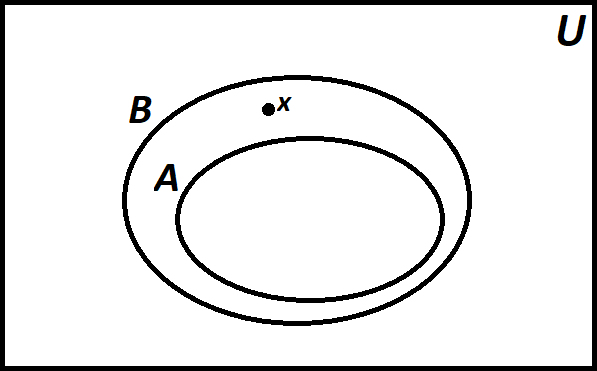
\includegraphics[width = 7 cm]{figures/sets/fig-sets-02-00.png}
      \caption{O conjunto $A$ está contido no conjunto $B$, equivalentemente, $B$ contém $A$.}
      \label{fig:sets-02-00}
  \end{figure}

  \textbf{Interseção:} Se estamos interessados em conjuntos/elementos que pertencem simultaneamente a dois conjuntos $A$ e $B$, dizemos que estamos interessados na interseção de $A$ e $B$ (denotada como $A \cap B$)$^{\ref{fig:sets-02-01}}$.
  
  \begin{figure}[hbt!]
      \centering      
      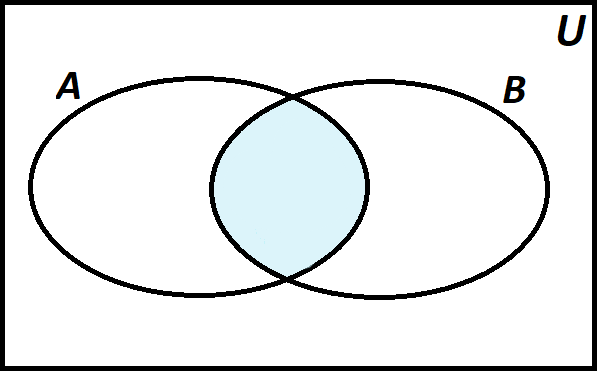
\includegraphics[width = 7 cm]{figures/sets/fig-sets-02-01.png}
      \caption{A região azul representa a visualização da interseção dos conjuntos $A$ e $B$.}
      \label{fig:sets-02-01}
  \end{figure}
  
  \textbf{União:} Já se estamos interessados nos conjuntos/elementos que fazem parte de $A$ ou de $B$ dizemos que, nosso objetivo é a união de $A$ e $B$ ($A \cup B$)$^{\ref{fig:sets-02-02}}$.
  
  \begin{figure}[hbt!]
      \centering      
      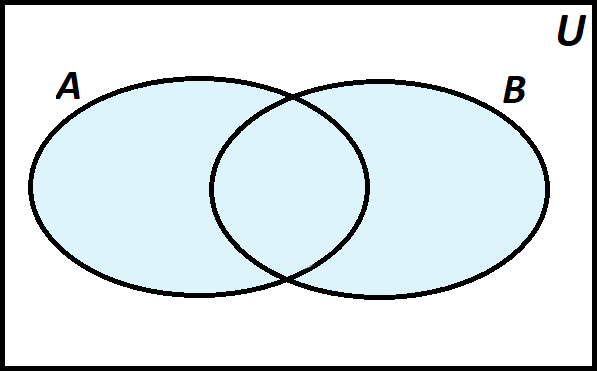
\includegraphics[width = 7 cm]{figures/sets/fig-sets-02-02.png}
      \caption{A região azul representa a visualização da união dos conjuntos $A$ e $B$.}
      \label{fig:sets-02-02}
  \end{figure}
  
  \textbf{Universo:} Quando estamos trabalhando com conjuntos é comum definirmos quem é nosso universo ($ \mathcal U $), isto é, o conjunto que conterá todos os conjuntos/elementos que estaremos trabalhando em um contexto$^{\ref{fig:sets-02-03}}$. Por exemplo, na reta real nosso universo é $\mathcal U = \mathbb{R}$.
  
  \begin{figure}[hbt!]
      \centering      
      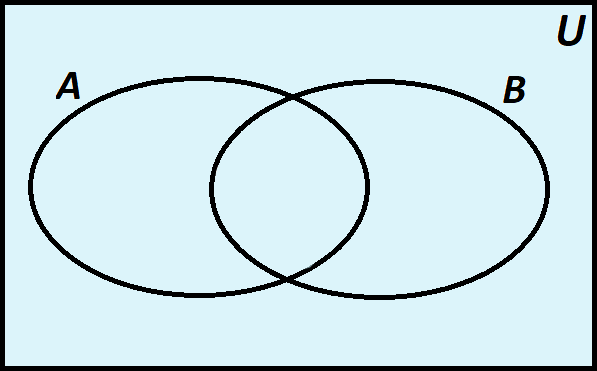
\includegraphics[width = 7 cm]{figures/sets/fig-sets-02-03.png}
      \caption{A região azul representa a visualização do nosso Universo.}
      \label{fig:sets-02-03}
  \end{figure}
  
  \textbf{Conjunto Complementar:} Sendo $A$ um conjunto, dizemos que o conjunto $A$ complementar ou complemento de $A$ (denotado como $\overline A$ ou $A^C$)contém todos os conjuntos/elementos que não estão contidos/pertencem a $A$, mas fazem parte de nosso universo ($\mathcal U$)$^{\ref{fig:sets-02-04}}$.
  
  \begin{figure}[hbt!]
      \centering      
      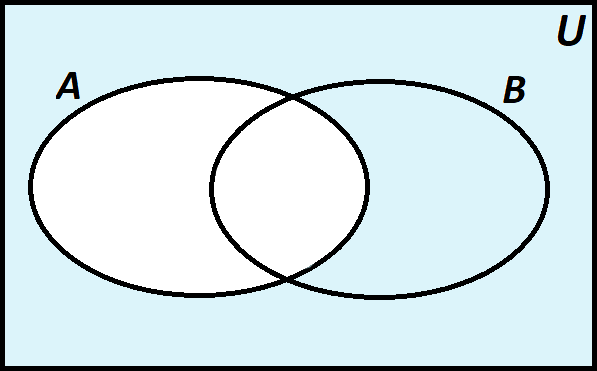
\includegraphics[width = 7 cm]{figures/sets/fig-sets-02-04.png}
      \caption{A região azul representa a visualização do complemento de $A$.}
      \label{fig:sets-02-04}
  \end{figure}
  
  \textbf{Diferença de Conjuntos :} Quando temos dois conjuntos e nosso objetivo são os conjuntos/elementos que pertencem a um destes conjuntos, mas não do outro dizemos que estamos interessados na diferença destes conjuntos. No caso, se quero os conjuntos/elementos de $B$, mas não queremos pegar os que também pertencem a $A$, queremos os elementos/conjuntos que pertencem a diferença de $B$ com $A$ (denotamos como $B-A$ ou $B \backslash A$)$^{\ref{fig:sets-02-05}}$.
  
  \begin{figure}[hbt!]
      \centering      
      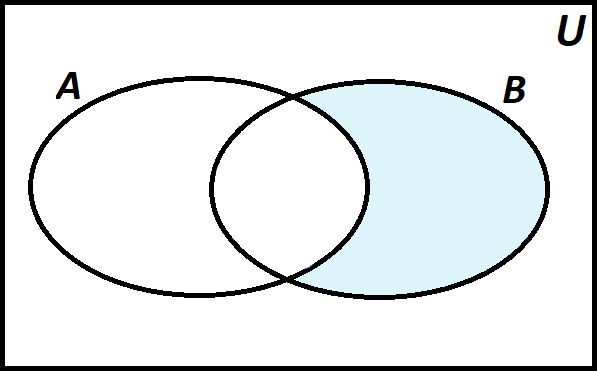
\includegraphics[width = 7 cm]{figures/sets/fig-sets-02-05.png}
      \caption{A região azul representa a visualização da diferença entre os conjuntos $B$ e $A$, isto é, a área onde estão os elementos que pertencem a $B$, mas não pertencem a $A$.}
      \label{fig:sets-02-05}
  \end{figure}
  
  Lembre-se: os diagramas apresentados servem como ferramenta auxiliar para ajudar a entender os conceitos, mas não devem ser vistos como a única ferramenta para compreender as definições e  a teoria exposta.
    
  \subsection{Definições}
  Seja $A$ e $B$ conjuntos ($\mathcal{U}$ nosso universo e $\emptyset$ o conjunto vazio, como definidos anteriormente). Assim temos, formalmente:

  \begin{itemize}
    \item \textbf{Diferença}: $A \backslash B = \{x | x \in A \land x \notin B\}$
  
    \item \textbf{Complementar}: $\overline A = \mathcal{U} \backslash A = \{x | x \in \mathcal{U} \land x \notin A\}$
  \end{itemize} 

  \subsection{Axiomas}
  Agora iremos apresentar alguns axiomas que servirão como base para todo o desenvolvimento dos conteúdos aqui propostos. Quando utilizarmos a palavra elemento, estaremos utilizando-a com a ideia de que um conjunto que pertença a outro é um elemento do segundo, para evitar repetir o uso excessivo da palavra conjunto.
  
  \textbf{Axioma da Completude:} Dois conjuntos são iguais, se e somente se, todo elemento que pertence ao primeiro conjunto pertence ao segundo e, todo elemento que pertence ao segundo também pertence ao primeiro, ou seja:
  
  \[\forall A \hspace{1.5mm} \forall B \hspace{1.5mm} (A = B) \iff (\forall x \hspace{1.5mm} (x \in A \iff x \in B))\] 
  
  Através desse axioma fica mais claro de entender duas propriedades dos conjuntos. 
  
  Deste axioma, vem a explicação do motivo de que a ordem dos elementos de um conjunto não importa. Pois dado dois conjuntos com os mesmos elementos, mas em ordem diferente (por exemplo, $X=\{a,b,c,d,e,f\}$ e o conjunto $Y=\{e,c,f,b,a,d\}$) eles ainda satisfazem a propriedade de que se $t$ pertence a um deles implica $t$ pertencer ao outro. Outro ponto interessante é que não importa se um conjunto possui elementos repetidos ele continuará igual ao que possui apenas um elemento, isto é, $X=\{a,b,d,e\}$ é igual ao $Y=\{b,a,d,a,e,b,b\}$. Ou seja, em um conjunto não importa a ordem e nem as repetições de elementos.
  
  \textbf{Axioma da Existencia do Conjunto Vazio: } Diremos que no nosso universo ($\mathbb{U}$), existe um conjunto tal que ele não contém ninguém, ou seja, ele é vazio, daí seu nome, Conjunto Vazio (denotado por $\emptyset$). O axioma é:
      
    \[\exists A \hspace{1.5mm} \forall x \hspace{1.5mm} \neg\hspace{0.5mm} (x \in A)\]
  
  \textbf{Unicidade do Conjunto Vazio}
  
  Podemos provar a unicidade do conjunto vazio a partir dos dois axiomas acimas, suponhamos que existam dois conjuntos ($A$ e $B$) com a propriedade do conjunto vazio, assim utilizando o axioma da Extensão concluíremos que eles são iguais, suponhamos $t$ arbitrário:
  
  \begin{center}
      \begin{landscape}
      \AxiomC{$\forall a  \forall b  (a = b) \iff (\forall x  (x \in a \iff x \in b))$}
      \UnaryInfC{$(A = B) \iff (\forall x  (x \in A \iff x \in B))$}
      \AxiomC{$t \in A $}
      \AxiomC{}
      \RightLabel{\scriptsize $1$}
      \UnaryInfC{$\forall x \neg (x \in A)$}
      \UnaryInfC{$\neg (t \in A)$}
      \BinaryInfC{$\perp$}
      \UnaryInfC{$t \in B$}
      \AxiomC{$t \in B$}
      \AxiomC{}
      \RightLabel{\scriptsize $1$}
      \UnaryInfC{$\forall x \neg (x \in B)$}
      \UnaryInfC{$\neg (t \in B)$}
      \BinaryInfC{$\perp$}
      \UnaryInfC{$t \in A$}
      \RightLabel{\scriptsize $\iff I_1$}
      \BinaryInfC{$t \in A \iff t \in B$}
      \UnaryInfC{$\forall x  (x \in A \iff x \in B)$}
      %\RightLabel{\scriptsize $\to E_4$}
      \BinaryInfC{A=B}
      \DisplayProof
      \end{landscape}
  \end{center}

  \textbf{Axioma do Par: } Este axioma nos diz que para todos os conjuntos $A$ e $B$, existe um conjunto conjunto que é $\{A,B\}$. Ou seja,
  
    \[\forall A \hspace{1.5mm} \forall B \hspace{1.5mm} \exists C \hspace{1.5mm} \forall x \hspace{1.5mm} (x \in C \leftrightarrow x = A \vee x = B)\]
      
  Vale ressaltar que se $A=B$, teremos $\{A,B\}=\{A,A\}=\{A\}$. A aplicação sucessiva deste axioma nos permite criar uma infinidade de conjuntos finitos. Por exemplo, $A=\emptyset$ e seja $B=\emptyset$, assim teremos $\{\emptyset\}$, sendo $B=\{\emptyset\}$, teremos agora $\{\emptyset,\{\emptyset\}\}$, agora fazendo $A=\{\emptyset\}$, teremos $\{\{\emptyset\}\}$.
  
  Não pretendemos nos aprofundar mais nos axiomas de conjuntos, dado que eles utilizarão conceitos abordados futuramente, nos capítulos de Relações, Funções e Axiomas.
  
  Mas como se pode ver em ..., podemos reduzir uma grande gama de coisas a conjuntas, assim podemos tratá-las na Teoria dos Conjuntos. Para saber mais sobre Teoria dos Conjuntos dê uma olhada em ... .

\section{Diagrama de Venn}
A maneira mais simples de entender a Teoria de Conjuntos, talvez seja o Diagrama de Venn. Criado por John Venn em 1880, esse sistema de representar graficamente conjuntos auxilia imensamente quem está começando a aprender esse assunto, principalmente para entender sobre a parte inicial de notações. Basicamente, consiste em representar num plano, o universo $\mathcal U$ como sendo um retângulo e cada conjunto $A,B,...$ como uma curva fechada simples (geralmente, círculo).
    
  \subsection{Para 1 ou 2 conjuntos}
  Começando com a ideia mais simples, a imagem abaixo representa em vermelho o conjunto $A$ dentro do universo $\mathcal U$:
  
  %\begin{figure}[h!]
  %    \centering
  %    \includegraphics{fig_set_01_01.png}
  %    \caption{Conjunto $A$ dentro de $\mathcal U$}
  %    \label{fig:fig_set_01_01}
  %\end{figure}
  
  Já sobre o conjunto complementar $A^c$, ele simplesmente é a parte que está no retângulo, mas não está no círculo, justamente o que não estava de vermelho na figura anterior.
  
  %\begin{figure}[h!]
  %    \centering
  %    \includegraphics{fig_set_01_02.png}
  %    \caption{Conjunto complementar $A^c$}
  %    \label{fig:fig_set_01_02}
  %\end{figure}
  
  Para representar que um elemento pertence ao conjunto $A$, simplesmente colocamos ele dentro do espaço delimitado pelo círculo que representa o conjunto, e para representar que um elemento nāo pertence ao conjunto $A$, fazemos o inverso.
  
  
  %\begin{figure}[h!]
  %    \centering
  %    \includegraphics{figure_set_01_03.png}
  %    \caption{$a \in A$ e $b \notin A$}
  %    \label{fig:figure_set_01_03}
  %\end{figure}
  
  Quando vamos representar mais de um conjunto em um diagrama de Venn, devemos necessariamente ter todas as possíveis relações, mas o que isso significa? Por exemplo, quando temos $2$ conjuntos $A$ e $B$, significa que devemos ter $4$ regiões representando respectivamente: elementos que pertencem somente à $A$, elementos que pertencem somente à $B$, elementos que pertencem à $A$ e à $B$ simultaneamente e elementos que não pertencem a nenhum dos conjuntos. Precisamos disso, para que tudo que provarmos para dois conjuntos $A$ e $B$, possa ser generalizado para dois conjuntos quaisquer, isso será explicado melhor num exemplo posterior.
  
  Utilizando esse artífiico, podemos representar todas as definições de intersecçāo, uniāo e diferença de $2$ conjuntos, introduzidas na seçāo anterior. Veja nas figuras abaixo:
  
  %\begin{figure}[h!]
  %    \centering
  %    \includegraphics{figure_set_01_04.png}
  %    \caption{Intersecção $A \cap B$}
  %    \label{fig:figure_set_01_04}
  %\end{figure}
  
  %\begin{figure}[h!]
  %    \centering
  %    \includegraphics{figure_set_01_05.png}
  %    \caption{União $A \cup B$}
  %    \label{fig:figure_set_01_05}
  %\end{figure}
  
  %\begin{figure}[h!]
  %    \centering
  %    \includegraphics{figure_set_01_06.png}
  %    \caption{Diferença $A \setminus B$}
  %    \label{fig:figure_set_01_06}
  %\end{figure}
  
  Todavia, isso ainda não permite fazer tudo que desejamos. Se quisermos representar que $A \subseteq B$, a ideia inicial seria colocar o círculo $A$ dentro do círculo $B$, quebrando o rigor de manter todas as possíveis relações, pois não teremos uma região para representar os elementos que pertecem somente a $A$. Então, como resolver esse problema? Representamos os conjuntos $A$ e $B$ da mesma forma que anteriormente e também escrevemos o símbolo do conjunto vazio $\emptyset$ na região dos elementos que pertencem somente a $A$. Assim, só existem elementos no conjunto $A$ que estão na região $A\cap B$, ou seja, se um elemento está em $A$, como consequência ele está em $B$, exatamente a definição de $A \subseteq B$.
  
  %\begin{figure}[h!]
  %    \centering
  %    \includegraphics{figure_set_01_07.png}
  %    \caption{Subconjunto $A \subseteq B$}
  %    \label{fig:figure_set_01_07}
  %\end{figure}
  
  É inegável que para muitos exemplos isso se torna inviável, principalmente quando o único objetivo é fazer uma ilustração matemática do problema, como por exemplo: tomamos o universo $\mathcal U$ como a fauna do nosso planeta, nele temos dois conjuntos $A$ de humanos e $B$ de mamíferos. É previamente conhecido que todos os humanos são mamíferos, falando de outra forma, que $A \subseteq B$. Logo, pra representar um problema que envolva esses elementos, podemos utilizar o \textbf{Diagrama de Euler}, similar ao Diagrama de Venn, com a diferença de que não é necessário mostrar todas as possíveis relações, mas apenas as relações específicas do problema retratado. E assim, fazer exatamente o que tinha sido proposto no parágrafo anterior e, colocar o círculo $A$ dentro do círculo $B$.

  %\begin{figure}[h!]
  %    \centering
  %    \includegraphics{figure_set_01_08.png}
  %    \caption{Diagrama de Euler $A \subseteq B$}
  %    \label{fig:figure_set_01_08}
  %\end{figure}

  \subsection{Para 3 conjuntos ou mais}    
  Já foi bastante falado sobre Diagrama de Venn, mas nem chegamos a trabalhar com mais de $2$ conjuntos, o que é importante, dado que a Teoria de Conjuntos não se resume a $A$ e $B$. Mas antes de partirmos para mais conjuntos, vamos pensar numa generalização de quantas regiões diferentes devemos ter para que o diagrama seja um Diagrama de Venn. Dado $n$ conjuntos diferentes, tomamos um elemento qualquer $x$, e para cada um dos $n$ conjuntos existem duas possibilidades: $x \in $ conjunto e $x \notin $ conjunto. Logo, concluímos que existem $\underbrace{\begin{matrix} 2\cdot2\cdots2\cdot2\end{matrix}}_{n} = 2^n$ possibilidades de pertencimento de $x$ nos conjuntos, equivalente à dizer que existem $2^n$ regiões diferentes. Isso bate perfeitamente com o caso anterior pra $2$ conjuntos, pois vimos que era necessário ter $4=2^2$ regiões diferentes.

  Agora, com $3$ conjuntos $A$, $B$ e $C$, o número de regiões diferentes é $2^3=8$, mas como iremos representá-las? A primeira ideia que vem a cabeça é adicionar um círculo representando o conjunto $C$ no diagrama da figura $\ref{fig:sets-02-00}$, intersectando as regiões já existentes, resultando na figura abaixo:

  Fazendo uma rápida contagem, obtemos $8$ regiões diferentes, exatamente como deve ser (lembrete: A região fora dos conjuntos mas dentro do universo $\mathcal U$, também é considerada na contagem). E da mesma forma que representamos bla bla bla

  \subsection{Aplicações}
  Ainda vai ter algo escrito

\section{Prova de Teoremas}
Nesta seção iremos tratar de formalizar definições e Teoremas. Ao contrário da seção $5.2$, onde o foco era transmitir a notação e uma ideia geral dos conceitos.

Aqui serão apresentadas algumas provas em Lean para o conteúdo apresentado. Não se preocupe, caso não entenda sobre o que o código quer dizer ignore ele por enquanto e após ler as próximas duas seções (que falam de conjuntos em Lean), volte e tente compreender o que foi feito. Já que o foco principal nesta parte são as provas matemáticas tradicionais e as definições mais precisas.

  \subsection{Prova Matemática Formal}
  Ainda vai ter algo escrito aqui

  \subsection{Dedução Natural}
  Ainda vai ter algo escrito aqui

\section{Conjuntos em Lean}
Embora na teoria axiomática dos conjuntos se considere conjuntos de objetos distintos, em matemática é mais comum considerar subconjuntos de algum dominio fixo ($\mathcal U $). É assim que os conjuntos são tratados em Lean. Para qualquer dado do tipo $U$, Lean nos retorna um novo dado tipo $conjunto$ $U$, que consiste no conjunto dos elementos de $U$. Assim, por exemplo, podemos raciocinar sobre conjuntos de números naturais, conjuntos de números inteiro ou conjuntos de pares de números naturais.

  \subsection{Notações}
  O lean possui uma biblioteca padrão para lidar com conjuntos chamada set e, sempre que formos utilizar um comando que pertence à ela, é necessário escrever {\fontencoding{U}\fontfamily{cmtt}\selectfont set.comando}. Entretanto, pra facilitar nossa vida, podemos escrever {\fontencoding{U}\fontfamily{cmtt}\selectfont open set} no início do código, o que permite escrevermos somente {\fontencoding{U}\fontfamily{cmtt}\selectfont comando}, e o lean já entende que ele pertence a biblioteca set.
  
  Além disso, para trabalharmos com conjuntos, também é essencial definirmos um tipo {\fontencoding{U}\fontfamily{cmtt}\selectfont U} e sabermos utilizar conjuntos e elementos desse tipo. Para isso, utilizamos o código abaixo:

  \begin{lstlisting}
  open set

  variable {U : Type}
  variables A B C : set U
  variable x : U \end{lstlisting}

  Temos aqui uma pequena lista de como se representa os principais caractéres da parte de conjuntos em Lean: 

  \begin{itemize}
      \item $\in$ $\rightarrow$ $\backslash$in
    
      \item $\notin$ $\rightarrow$ $\backslash$notin
    
      \item $\subset$ $\rightarrow$ $\backslash$subset
    
      \item $\subseteq$ $\rightarrow$ $\backslash$sub
    
      \item $\emptyset$ $\rightarrow$ $\backslash$empty
    
      \item $\cup$ $\rightarrow$ $\backslash$un \ ou \ $\backslash$cup \ ou \ $\backslash$union
    
      \item $\cap$ $\rightarrow$ $\backslash$i \ ou \ $\backslash$cap \ ou \ $\backslash$intersection
  \end{itemize}

  Obs$^{1}$.: O conjunto universal é denotado {\fontencoding{U}\fontfamily{cmtt} \selectfont univ}.

  Obs$^{2}$.: O complementar de um conjunto é denotado com um símbolo de negação antes de seu símbolo, assim: $-A$

  Podemos ver alguns exemplos abaixo:
  \begin{lstlisting}
    open set
    variable {U : Type}
    variables A B C : set U
    variable x : U

    #check x ∈ A
    #check A ∪ B
    #check B \ C
    #check C ∩ A
    #check -C
    #check ∅ ⊆ A
    #check B ⊆ univ \end{lstlisting}

  Noções básicas da teoria dos conjuntos são definidas na biblioteca principal do Lean, mas teoremas e notações adicionais que iremos utilizar nesse capítulo, estão disponíveis em uma biblioteca auxiliar que é carregada com o comando 
  {\fontencoding{U}\fontfamily{cmtt} \selectfont import data.set}, o qual deve aparecer no início do arquivo.

  \begin{lstlisting}
    import data.set
    open set
    variable {U : Type}
    variables A B C : set U
    variable x : U \end{lstlisting}

  A partir desse momento, para evitar repetição, iremos omitir as $4$ primeiras linhas do código, no entanto \textbf{você deve lembrar que elas existem para seu código funcionar.} Já sobre a linha $5$, não é necessário escrever nos próximos exemplos, pois sempre iremos se referenciar a um elemento do tipo{\fontencoding{U}\fontfamily{cmtt} \selectfont U}, dentro de {\fontencoding{U}\fontfamily{cmtt}\selectfont example, lemma} ou {\fontencoding{U}\fontfamily{cmtt}\selectfont theorem}.

  \subsection{Primeiros Passos}

  Relembrando a definição de subconjunto, podemos utilizar o template abaixo para mostrar que o conjunto $A$ é um subconjunto de $B$:

  \begin{lstlisting}
  example : A ⊆ B :=
  assume x : U,
  assume h : x ∈ A,
  show x ∈ B, from sorry \end{lstlisting}

  Obs: Na linha $2$ poderíamos ter escrito somente {\fontencoding{U}\fontfamily{cmtt}\selectfont assume x}, pois já inferiria que {\fontencoding{U}\fontfamily{cmtt}\selectfont x} é do tipo {\fontencoding{U}\fontfamily{cmtt}\selectfont U}.

  Já para mostrar que $A$ e $B$ são iguais, temos dois comandos diferentes: {\fontencoding{U}\fontfamily{cmtt}\selectfont eq\_of\_subset\_of\_subset} e {\fontencoding{U}\fontfamily{cmtt}\selectfont ext}.

  \textbf{eq\_of\_subset\_of\_subset:} Ele funciona interpretando a seguinte expressão $(A \subseteq B \wedge B \subseteq A) \Rightarrow A=B$, ou seja, obtém a equivalência dos conjuntos a partir do fato de que o primeiro é subconjunto do segundo, e vice-vera. Veja o código:

  \begin{lstlisting}
  example : A = B :=
  eq_of_subset_of_subset
    (assume x,
      assume h : x ∈ A,
      show x ∈ B, from sorry)
    (assume x,
      assume h : x ∈ B,
      show x ∈ A, from sorry) \end{lstlisting}

  \textbf{ext:} É uma sigla para ``extensionality", ou seja, extensionalidade. Matemáticamente, isso representa a expressão $\forall x \ (x \in A \leftrightarrow x \in B) \Rightarrow A=B$. Veja o código:

  \begin{lstlisting}
  example : A = B :=
  ext (assume x, iff.intro
    (assume h : x ∈ A,
      show x ∈ B, from sorry)
    (assume h : x ∈ B,
      show x ∈ A, from sorry)) \end{lstlisting}

  Além disso, o Lean possui interpretação ambígua para regras de união, interseção e outras operações em conjuntos que são consideradas “definições”. Isso significa que as expressões $x$ $\in$ $A$ $\cap$ $B$ e $x$ $\in$ $A$ $\wedge$ $x$ $\in$ $B$ possuem a mesma interpretação no Lean. Isso também é válido para outras construções em conjuntos, como: $x$ $\in$ $A$ $\backslash $ $B$ e $x$ $\in$ $A$ $\wedge$ $\neg$ $(x$ $\in$ $B)$. O termo $\neg$ $(x$ $\in$ $B)$ é somente outra forma de escrever $x$ $\notin$ $B$. Abaixo são apresentadas algumas aplicações dessa interpretação:

  \begin{lstlisting}
  example : ∀ x, x ∈ A → x ∈ B → x ∈ A ∩ B :=
  assume x,
  assume h₁ : x ∈ A,
  assume h₂ : x ∈ B,
  show x ∈ A ∩ B, from and.intro h₁ h₂

  example : A ⊆ A ∪ B :=
  assume x,
  assume h : x ∈ A,
  show x ∈ A ∪ B, from or.inl h

  example : ∅ ⊆ A  :=
  assume x,
  assume h : x ∈ (∅ : set U),
  show x ∈ A, from false.elim h \end{lstlisting}

  Observe no último exemplo a necessidade de usar a notação {\fontencoding{U}\fontfamily{cmtt} \selectfont ($\emptyset$ : set U)}, dizendo ao nosso provador que o $\emptyset$ é um conjunto de {\fontencoding{U}\fontfamily{cmtt}
  \selectfont U}. Isso acontece pois ele não consegue inferir que tipo é o conjunto vazio, dado que por definição, esse conjunto existe em qualquer universo, ou seja, pode ser de qualquer tipo.

  Opcionalmente, podemos usar alguns teoremas da biblioteca {\fontencoding{U}\fontfamily{cmtt}
  \selectfont data.set}, projetados especificamente para uso em conjuntos:

  \begin{lstlisting}
  example : ∀ x, x ∈ A → x ∈ B → x ∈ A ∩ B :=
  assume x,
  assume : x ∈ A,
  assume : x ∈ B,
  show x ∈ A ∩ B, from mem_inter ‹x ∈ A› ‹x ∈ B›

  example : A ⊆ A ∪ B :=
  assume x,
  assume h : x ∈ A,
  show x ∈ A ∪ B, from mem_union_left B h

  example : ∅ ⊆ A  :=
  assume x,
  assume : x ∈ ∅,
  show x ∈ A, from absurd this (not_mem_empty x) \end{lstlisting}

  Lembre-se que o comando{\fontencoding{U}\fontfamily{cmtt}
  \selectfont absurd} pode ser usado para provar qualquer fato a partir de duas hipóteses contrárias: $h_1$ : $P$ e $h_2$ : $\neg$ $P$. 

  Aqui, o teorema {\fontencoding{U}\fontfamily{cmtt}
  \selectfont not\_mem\_empty x} significa $x$ $\notin$ $\emptyset$. Para ver a declaração de teoremas disponíveis, utilize o comando{\fontencoding{U}\fontfamily{cmtt}
  \selectfont \#check}:

  \begin{lstlisting}
  #check @mem_inter
  #check @mem_of_mem_inter_left
  #check @mem_of_mem_inter_right
  #check @mem_union_left
  #check @mem_union_right
  #check @mem_or_mem_of_mem_union
  #check @not_mem_empty \end{lstlisting}

  Neste caso, o símbolo{\fontencoding{U}\fontfamily{cmtt}
  \selectfont @} impede que ele tente preencher argumentos implícitos automaticamente, forçando-o a exibir a declaração completa do teorema.

  Já que podemos relacionar conjuntos com suas definições lógica, isso auxilia a comprovação de inclusões entre conjuntos:

  \begin{lstlisting}
  example : A \ B ⊆ A :=
  assume x,
  assume : x ∈ A \ B,
  show x ∈ A, from and.left this

  example : A \ B ⊆ -B :=
  assume x,
  assume : x ∈ A \ B,
  have x ∉ B, from and.right this,
  show x ∈ -B, from this \end{lstlisting}

  Novamente, é possível usar versões dos teoremas projetados especificamente para conjuntos:

  \begin{lstlisting}
  example : A \ B ⊆ A :=
  assume x,
  assume : x ∈ A \ B,
  show x ∈ A, from mem_of_mem_diff this

  example : A \ B ⊆ -B :=
  assume x,
  assume : x ∈ A \ B,
  have x ∉ B, from not_mem_of_mem_diff this,
  show x ∈ -B, from this \end{lstlisting}

  %Acho que a partir desse ponto, não é necessário ter nesse capítulo. Talvez seja melhor deixar só pro capítulo de propriedades. Por isso, já copiei e colei no outro capítulo. Se ainda sim quiser falar sobre como lidar com sorry, pegue algum dos exemplos já citados acima. E se quiser colocar mais coisas teóricas ou explicativas, está totalmente livre. Mas deixe as propriedades/identidades pro capítulo delas.

\section{Cálculo em Conjuntos}
Ainda vai ter algo escrito aqui

  \subsection{Cálculo Matemático}
  Ainda vai ter algo escrito aqui

  \subsection{Calc em Lean}
  Ainda vai ter algo escrito aqui

\section{Propriedades}
A seguir teremos algumas propriedades e a prova do porque estão corretas.
    
\begin{itemize}  
    \item $A \cup \overline A = \mathbb{U}$
\end{itemize} 

\textbf{Prova:} Seja $x$ um elemento de $A \cup \overline A$, assim temos que 
\[x \in (A \cup \overline A)\]
\[ \iff x \in A \vee x \in \overline A\]
    
\begin{itemize}
    \item $A \cap \overline A = \empty{U}$
\end{itemize} 

\textbf{Prova:} Seja $x$ um elemento de $A \cap \overline A$, assim:

$(i)$ Provaremos que $ \forall x (x \in A \cap \overline A) \rightarrow \forall x  (x \in \emptyset) $ :

\begin{center}
    \AxiomC{}
    \RightLabel{\scriptsize $1$}
    \UnaryInfC{$ \forall x (x \in A \cap \overline A)$}
    \UnaryInfC{$t \in A \cap \overline A$}
    \UnaryInfC{$t \in A \land t \in \overline A $}
    \UnaryInfC{$t \in A $}
    \AxiomC{}
    \RightLabel{\scriptsize $1$}
    \UnaryInfC{$ \forall x (x \in A \cap \overline A)$}
    \UnaryInfC{$t \in A \cap \overline A$}
    \UnaryInfC{$t \in A \land t \in \overline A $}
    \UnaryInfC{$t \in \overline A $}
    \UnaryInfC{$t \in \mathbb{U} \land t \notin A $}
    \UnaryInfC{$t \notin A $}
    \BinaryInfC{$\perp$}
    \UnaryInfC{$t \in \emptyset$}
    \UnaryInfC{$\forall x  (x \in \emptyset)$}
    \RightLabel{\scriptsize $1$}
    \UnaryInfC{$ \forall x (x \in A \cap \overline A) \rightarrow \forall x  (x \in \emptyset) $}
    \DisplayProof
\end{center}
    
$(ii)$ Provaremos que $ \forall x  (x \in \emptyset) \rightarrow \forall x (x \in A \cap \overline A)$ :
\begin{center}
    \AxiomC{}
    \RightLabel{\scriptsize $1$}
    \UnaryInfC{$\forall x  (x \in \emptyset)$}
    \UnaryInfC{$\perp$}
    \UnaryInfC{$t \in A \cap \overline A$}
    \UnaryInfC{$ \forall x (x \in A \cap \overline A)$}
    \RightLabel{\scriptsize $1$}
    \UnaryInfC{$\forall x  (x \in \emptyset) \rightarrow \forall x (x \in A \cap \overline A)$}
    \DisplayProof
\end{center}

Portanto, de $(i)$ e $(ii)$, concluímos que $ \forall x (x \in A \cap \overline A) \iff \forall x  (x \in \emptyset) $, ou seja, $A \cap \overline A$.

%Renan
Como o Lean tem que desenvolver definições, ele pode acabar se confundindo às vezes. Por exemplo, na prova a seguir, se você subtituir a última linha por{\fontencoding{U}\fontfamily{cmtt}
\selectfont sorry}, o Lean terá problemas tentando entender que você quer que ele desenvolva o símbolo de subconjunto:

\begin{lstlisting}
example : A ∩ B ⊆ B ∩ A :=
assume x,
assume h : x ∈ A ∩ B,
have h₁ : x ∈ A, from and.left h,
have h₂ : x ∈ B, from and.right h,
and.intro h₂ h₁ \end{lstlisting}

Uma solução alternativa é usar o comando{\fontencoding{U}\fontfamily{cmtt}
\selectfont show}. Na maioria das vezes, fornecer informações adicionais para o Lean pode ser útil. Outra solução é nomear um teorema, o que leva o Lean a usar um método um pouco diferente de processar a prova, corrigindo o problema como um efeito colateral de sorte.

\begin{lstlisting}
example : A ∩ B ⊆ B ∩ A :=
assume x,
assume h : x ∈ A ∩ B,
have h₁ : x ∈ A, from and.left h,
have h₂ : x ∈ B, from and.right h,
show x ∈ B ∩ A, from sorry

theorem my_example : A ∩ B ⊆ B ∩ A :=
assume x,
assume h : x ∈ A ∩ B,
have h₁ : x ∈ A, from and.left h,
have h₂ : x ∈ B, from and.right h,
sorry \end{lstlisting}

Parte de Identidade de Conjuntos: Nessa seção, falaremos brevemente sobre Identidades de conjuntos.

Iniciaremos com um exemplo simples: a regra da distributividade para conjuntos: $A \cup (B \cap C)$ = $(A \cup B) \cap (A \cup C)$. Uma maneira de prova-la é:


\begin{lstlisting}
import data.set
open set

variable {U : Type}
variables A B C : set U

example : A ∪ (B ∩ C) = (A ∪ B) ∩ (A ∪ C) :=
eq_of_subset_of_subset
  (assume x,
    assume h : x ∈ A ∪ (B ∩ C),
    or.elim h
      (assume h₁ : x ∈ A,
        have h₂ : x ∈ A ∪ B, from or.inl h₁,
        have h₃ : x ∈ A ∪ C, from or.inl h₁,
        show x ∈ (A ∪ B) ∩ (A ∪ C), from and.intro h₂ h₃)
      (assume h₁ : x ∈ B ∩ C,
        have h₂ : x ∈ B, from and.left h₁,
        have h₃ : x ∈ C, from and.right h₁,
        have h₄ : x ∈ A ∪ B, from or.inr h₂,
        have h₅ : x ∈ A ∪ C, from or.inr h₃,
        show x ∈ (A ∪ B) ∩ (A ∪ C), from and.intro h₄ h₅))
  (assume x,
    assume h : x ∈ (A ∪ B) ∩ (A ∪ C),
    have h₁ : x ∈ A ∪ B, from and.left h,
    have h₂ : x ∈ A ∪ C, from and.right h,
    or.elim h₁
      (assume h₃ : x ∈ A,
        show x ∈ A ∪ (B ∩ C), from or.inl h₃)
      (assume h₃ : x ∈ B,
      or.elim h₂
        (assume h₄ : x ∈ A,
        show x ∈ A ∪ (B ∩ C), from or.inl h₄)
        (assume h₄ : x ∈ C,
        have h₅ : x ∈ B ∩ C, from and.intro h₃ h₄, 
        show x ∈ A ∪ (B ∩ C), from or.inr h₅)))
\end{lstlisting}

Outra identidade que usaremos como exemplo aqui é a Lei de Absorção:  

\begin{center}
    $A \cup (A \cap B) = A$
\end{center}

Nos templates abaixo temos duas formas de escrever a prova: a que estamos utilizando ao longo deste capítulo; e em forma de lógica booleana, trocando o sinal de igual pelo de equivalência, ou ``se e somente se", ($\leftrightarrow$). (Você consegue reprentá-lo no Lean escrevendo: $\backslash$iff ou $\backslash$lr)

\begin{lstlisting}
import data.set
open set

theorem inter_subseq (H : Type)(P Q : set H) : P ∩ (P ∪ Q) = P :=
eq_of_subset_of_subset
  (assume x,
    assume h : x ∈ P ∩ (P ∪ Q),
    show x ∈ P, from h.left)
  (assume x,
    assume h : x ∈ P,
    have h₁ : x ∈ P ∪ Q, from or.inl h,
    show x ∈ P ∩ (P ∪ Q), from and.intro h h₁)

variable  U : Type
variables A B : set U

example : A ∪ (A ∩ B) = A :=
calc
  A ∪ (A ∩ B) = (A ∪ A) ∩ (A ∪ B) : by rw union_distrib_left
          ... = A ∩ (A ∪ B)       : by rw union_self
          ... = A                 : by rw inter_subseq
\end{lstlisting}

\begin{lstlisting}
import logic.basic
open classical

theorem left_of_and (P Q : Prop) : P ∧ (P ∨ Q) ↔ P :=
iff.intro
  (assume h : P ∧ (P ∨ Q),
  show P, from h.left)
  (assume h : P,
  have h₁ : P ∨ Q, from or.inl h,
  show P ∧ (P ∨ Q), from and.intro h h₁)

variables A B : Prop

example : A ∨ (A ∧ B) ↔ A :=
calc
  A ∨ (A ∧ B) ↔ (A ∨ A) ∧ (A ∨ B) : by rw or_and_distrib_left
          ... ↔ A ∧ (A ∨ B)        : by rw or_self
          ... ↔ A                  : by rw left_of_and
\end{lstlisting}

  \subsection{Básicas}
  %Pode ser separada em: Básicas, Sobre o conjunto vazio, Sobre o Universo
  Ainda vai ter algo escrito aqui

  \subsection{Comutatividade}
  Ainda vai ter algo escrito aqui

  \subsection{Associatividade}
  Ainda vai ter algo escrito aqui

  \subsection{Distributividade}
  Ainda vai ter algo escrito aqui

  \subsection{Complementar/Lei de Demorgan}
  Ainda vai ter algo escrito aqui

  \subsection{Lei da Absorção}
  Ainda vai ter algo escrito aqui

  \subsection{Extras}
  Ainda vai ter algo escrito aqui

\section{Famílias Indexadas}

  \subsection{Definição}
  Ainda vai ter algo escrito aqui

  \subsection{Em Lean}
  Ainda vai ter algo escrito aqui

\section{Power Set}

  \subsection{Definição}
  Ainda vai ter algo escrito aqui

  \subsection{Em Lean}
  Ainda vai ter algo escrito aqui

\section{Exercícios}
\begin{enumerate}
    
\item Questões de Identidades de conjuntos
    
\begin{lstlisting}
import data.set
open set

section
  variable U : Type
  variables A B C : set U

--Comutatividade em ∩ e ∪ 
  example : A ∩ B = B ∩ A := 
  eq_of_subset_of_subset
    (assume x,
        assume h : x ∈ A ∩ B,
        have h₁ : x ∈ A, from h.left,
        have h₂ : x ∈ B, from h.right,
        show x ∈ B ∩ A, from and.intro h₂ h₁)
    (assume x,
        assume h : x ∈ B ∩ A,
        have h₁ : x ∈ B, from h.left,
        have h₂ : x ∈ A, from h.right,
        show x ∈ A ∩ B, from and.intro h₂ h₁)

  example : A ∪ B = B ∪ A:=
  eq_of_subset_of_subset
    (assume x,
        assume h : x ∈ A ∪ B,
        or.elim h
        (assume h₁ : x ∈ A,
        show x ∈ B ∪ A, from or.inr h₁)
        (assume h₁ : x ∈ B,
        show x ∈ B ∪ A, from or.inl h₁))
    (assume x,
        assume h : x ∈ B ∪ A,
        or.elim h
        (assume h₁ : x ∈ B,
        show x ∈ A ∪ B, from or.inr h₁)
        (assume h₁ : x ∈ A,
        show x ∈ A ∪ B, from or.inl h₁))

--Associatividade
  example : (A ∩ B) ∩ C = A ∩ (B ∩ C) :=
  eq_of_subset_of_subset
    (assume x,
        assume h : x ∈ (A ∩ B) ∩ C,
        have h₁ : x ∈ A ∩ B, from h.left,
        have h₂ : x ∈ B ∩ C, from and.intro h₁.right h.right,
        show x ∈ A ∩ (B ∩ C), from and.intro h₁.left h₂) 
    (assume x,
        assume h : x ∈ A ∩ (B ∩ C),
        have h₁ : x ∈ B ∩ C, from h.right,
        have h₂ : x ∈ A ∩ B, from and.intro h.left h₁.left,
        show x ∈ (A ∩ B) ∩ C, from and.intro h₂ h₁.right) 

--De Morgan
  open classical 
  example : -(A ∩ B) = -A ∪ -B :=
    ext $
    assume x,
    iff.intro
        (assume h₁ : x ∈ -(A ∩ B),
            have g₁ : x ∈ (A ∪ -A), from em (x ∈ A),
            have g₂ : x ∈ (B ∪ -B), from em (x ∈ B),
            or.elim g₁
                (assume h₂ : x ∈ A, or.elim g₂
                    (assume h₃ : x ∈ B, show x ∈ -A ∪ -B,
                        from false.elim (h₁ ⟨h₂,h₃⟩))
                    (assume h₃ : x ∈ -B, show x ∈ -A ∪ -B,
                        from or.inr h₃))
                (assume h₂ : x ∈ -A, show x ∈ -A ∪ -B,
                    from or.inl h₂))

        (assume h₁ : x ∈ -A ∪ -B,
            assume h₂ : x ∈ (A ∩ B), show false,
            from or.elim h₁
                (assume h₃ : x ∈ -A, h₃ h₂.left )
                (assume h₃ : x ∈ -B, h₃ h₂.right))

  example : -(A ∪ B) = -A ∩ -B :=
    ext $
    assume x,
    iff.intro
        (assume h₁ : x ∈ -(A ∪ B),
            have g₁ : x ∈ -A, from
            assume h₂ : x ∈ A,
                have h₃ : x ∈ A ∪ B,
                from or.inl h₂, (h₁ h₃),
            have g₂ : x ∈ -B, from
            assume h₂ : x ∈ B,
                have h₃ : x ∈ A ∪ B,
                from or.inr h₂, (h₁ h₃),
            show x ∈ -A ∩ -B, from ⟨g₁, g₂⟩)

        (assume h₁ : x ∈ -A ∩ -B,
            show x ∈ -(A ∪ B), from
            assume h₂ : x ∈ A ∪ B,
            or.elim h₂
                (assume h3 : x ∈ A, h₁.left h3)
                (assume h3 : x ∈ B, h₁.right h3))
end 
\end{lstlisting}

\item Prove que $A \cup \overline A = \mathcal U$. (Fornecendo uma prova tradicional e uma em Lean.)

\textbf{Resposta} 




\item Questões com calc
    
    
\end{enumerate}
